\section{Timeplan}

\subsection{Time Management Towards the Deadline}

After the project kick-off at the beginning of February, the team intends on spending the entire month in the planning phase. We think
this is the right decision as it will allow us to carefully examine each aspect of our project, from the business standpoint, the requirements
and component structure to the security, release planning and post-launch maintenance. Such a time window will allow us to carry out a design sprint,
as well as prepare the following items before we can start the development stage:
\begin{itemize}
    \item Figma Prototype
    \item UML Component Diagram
    \item UML Context Diagram
    \item Excel Spreadsheet with Project Requirements, Time Estimations and MoSCoW Prioritization
    \item UML Data Model Diagram
    \item UML Class Diagram
    \item Business Model, along with Personas and Value Proposition Canvases
    \item UML Use Case Diagrams
    \item UML Sequence Diagrams
    \item UML State Machine Diagrams
\end{itemize}

Once the initial documentation phase is finished, the team will move onto the development phase which will last until the beginning
of May and will result in the delivery of the Minimum Viable Product for LinkedGym. Next, the team will spend the rest of May adding more features and polishing
the product to be ready for the realease of the Minimum Marketable Product at the beginning of June. At this point, the team will continue on adding features 
that have been prioritized as "Could", implementing user feedback and fixing any bugs that will pop up, but the project will move into the final, maintenance phase.
By reaching the final phase of the project, the Agile process will also be downscaled, which is described in the subsection *insert link to later subsection*.

\begin{figure}[H]
    \centering
    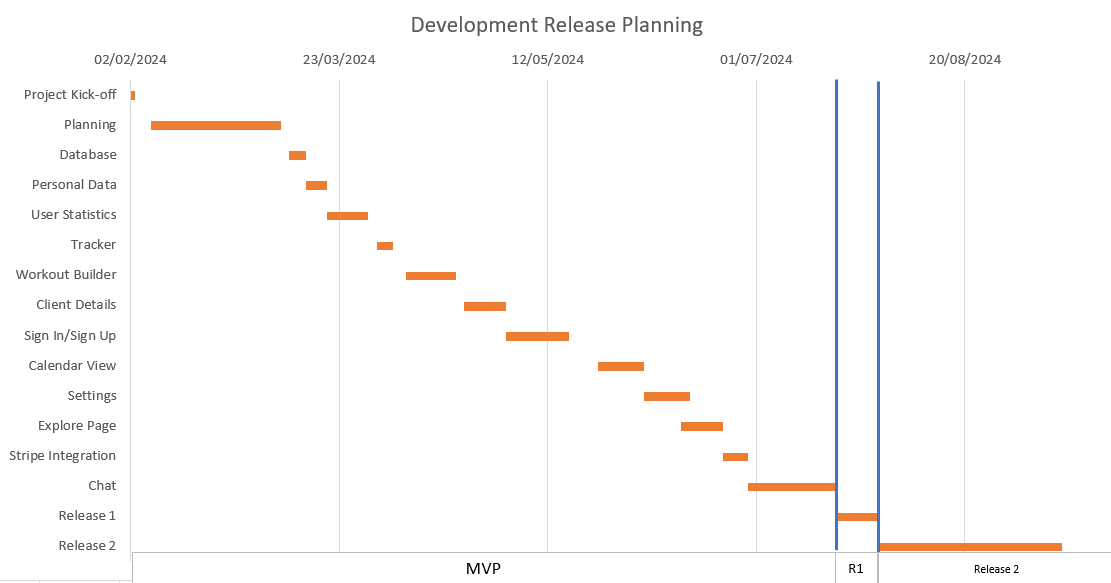
\includegraphics[width=0.8\textwidth]{images/initial_gantt_chart.png}
    \caption{First Version of the Timeplan Gantt Chart}
    \label{fig:initialganttchart}
\end{figure}

\begin{figure}[H]
    \centering
    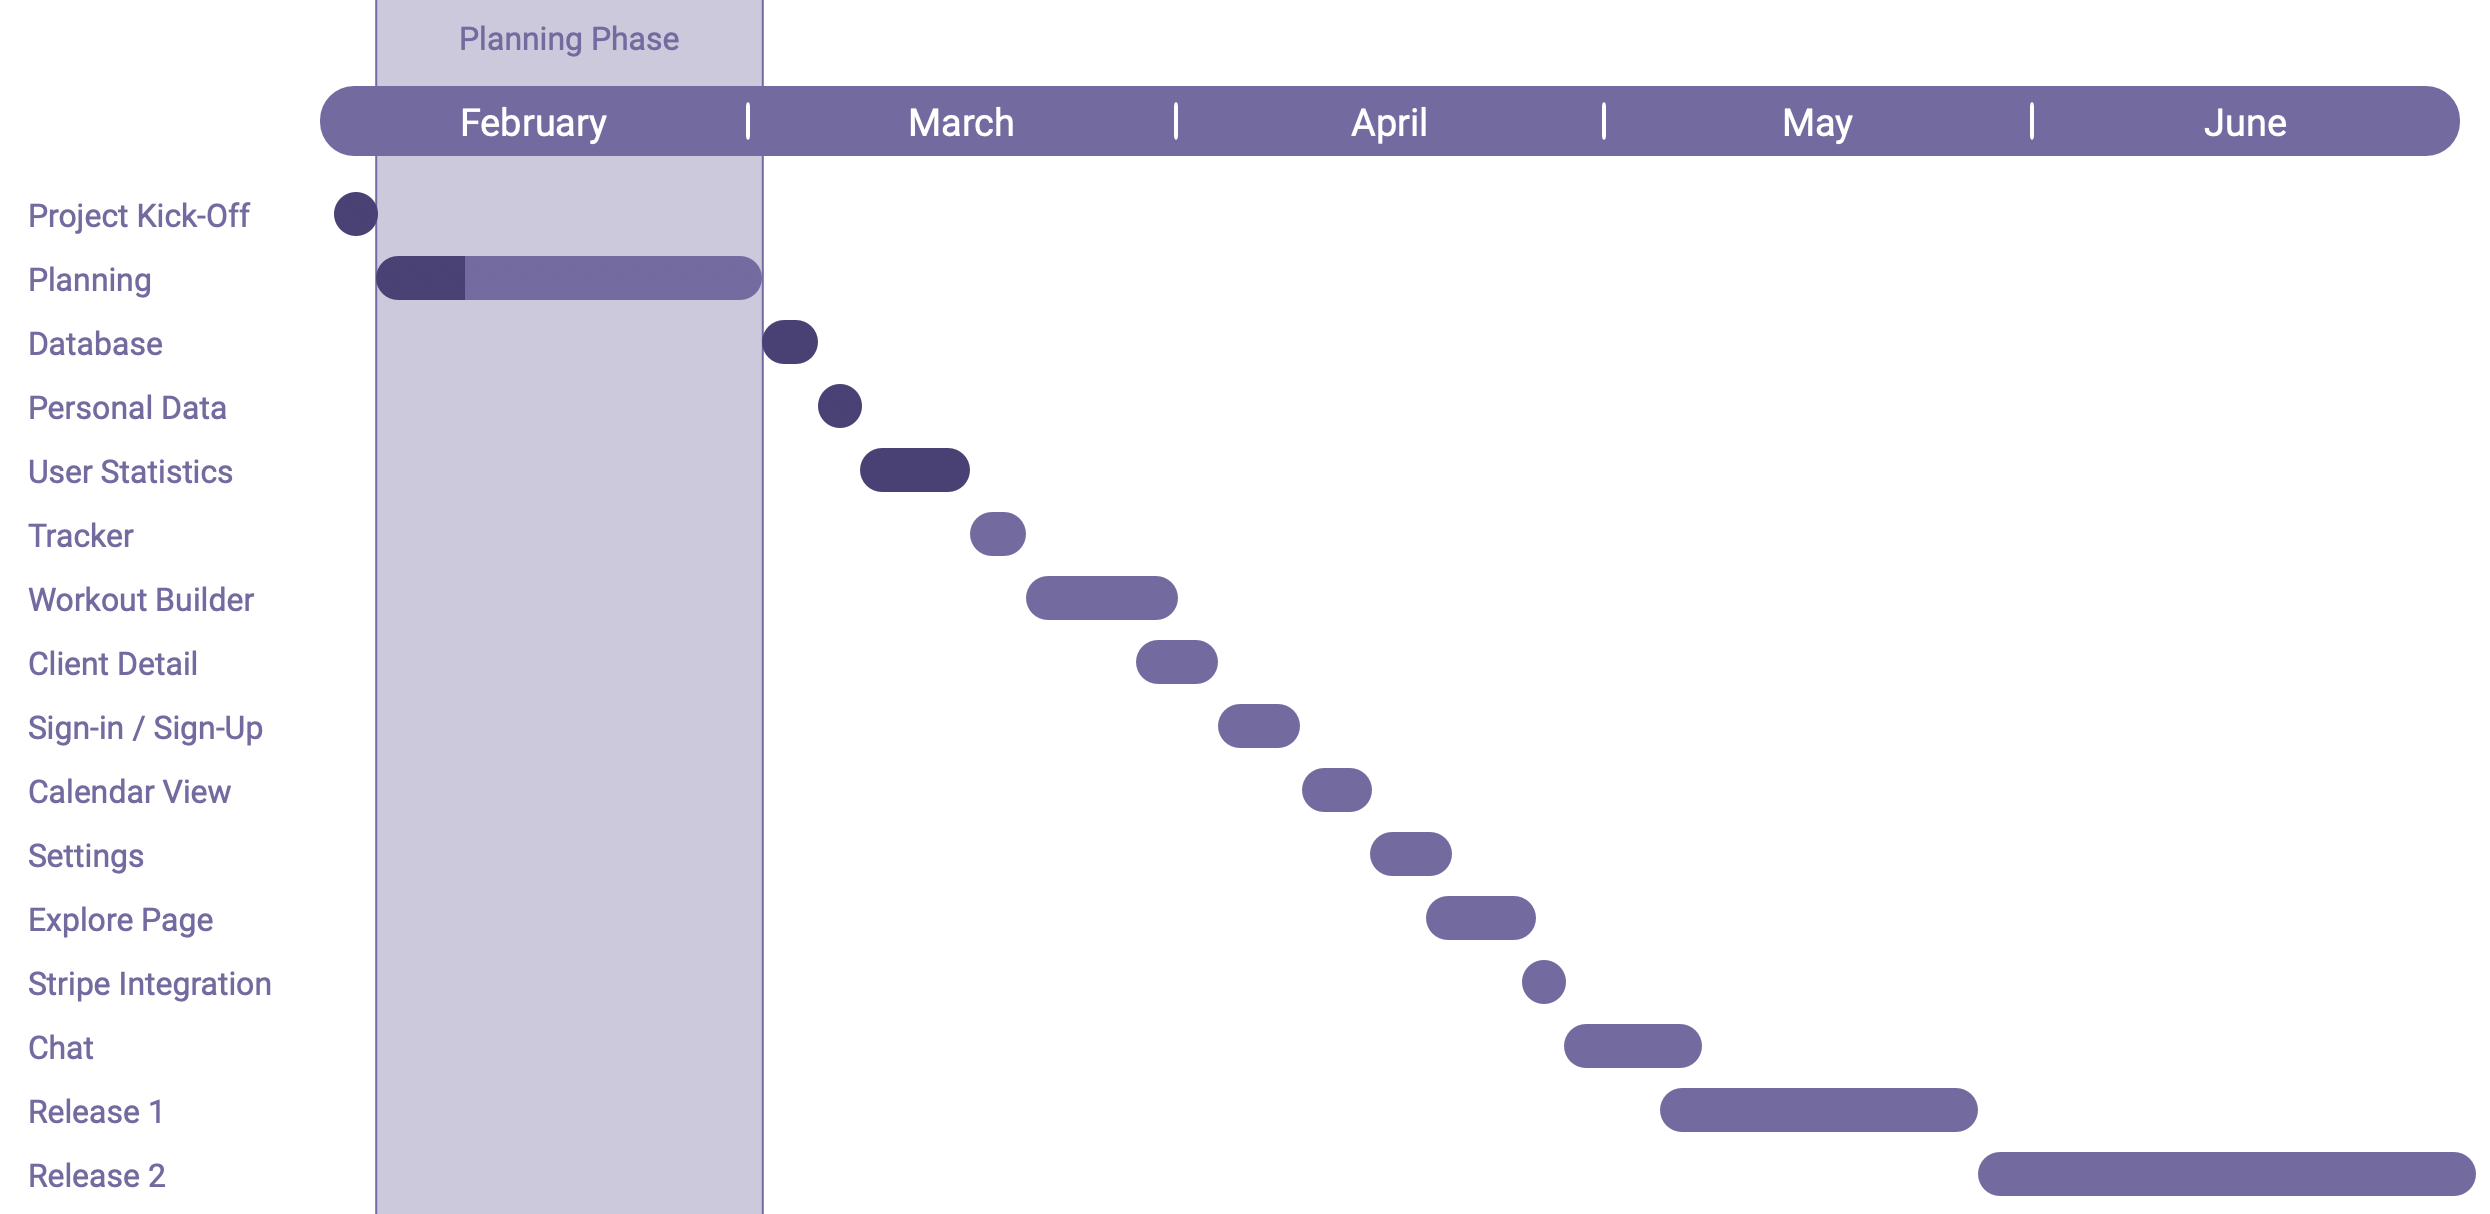
\includegraphics[width=0.8\textwidth]{images/gantt_chart.png}
    \caption{Second Version of the Timeplan Gantt Chart}
    \label{fig:ganttchart}
\end{figure}

\subsection{Time Estimates}
To prepare a Time Management plan as seen in the previous section, the team has conducted both a top-down, as well as a bottom-up 
time estimation for each requirement, to ensure our resutls are as accurate as possible. We went through this process twice during the
project, as we were not happy with the initial estimates we got. In the end, we are confident in our plan.
For the estimation process we used a Microsoft Excel Workbook, where each Spreadsheet corresponded to one component, and contained
all of it's requirements. As our estimation factor, we chose to use the number pi rounded up to two decimal places - 3,14. We also chose to
use MoSCoW prioritization for each requirement. The result of our work can be seen below in the attached print out of the spreadsheets.

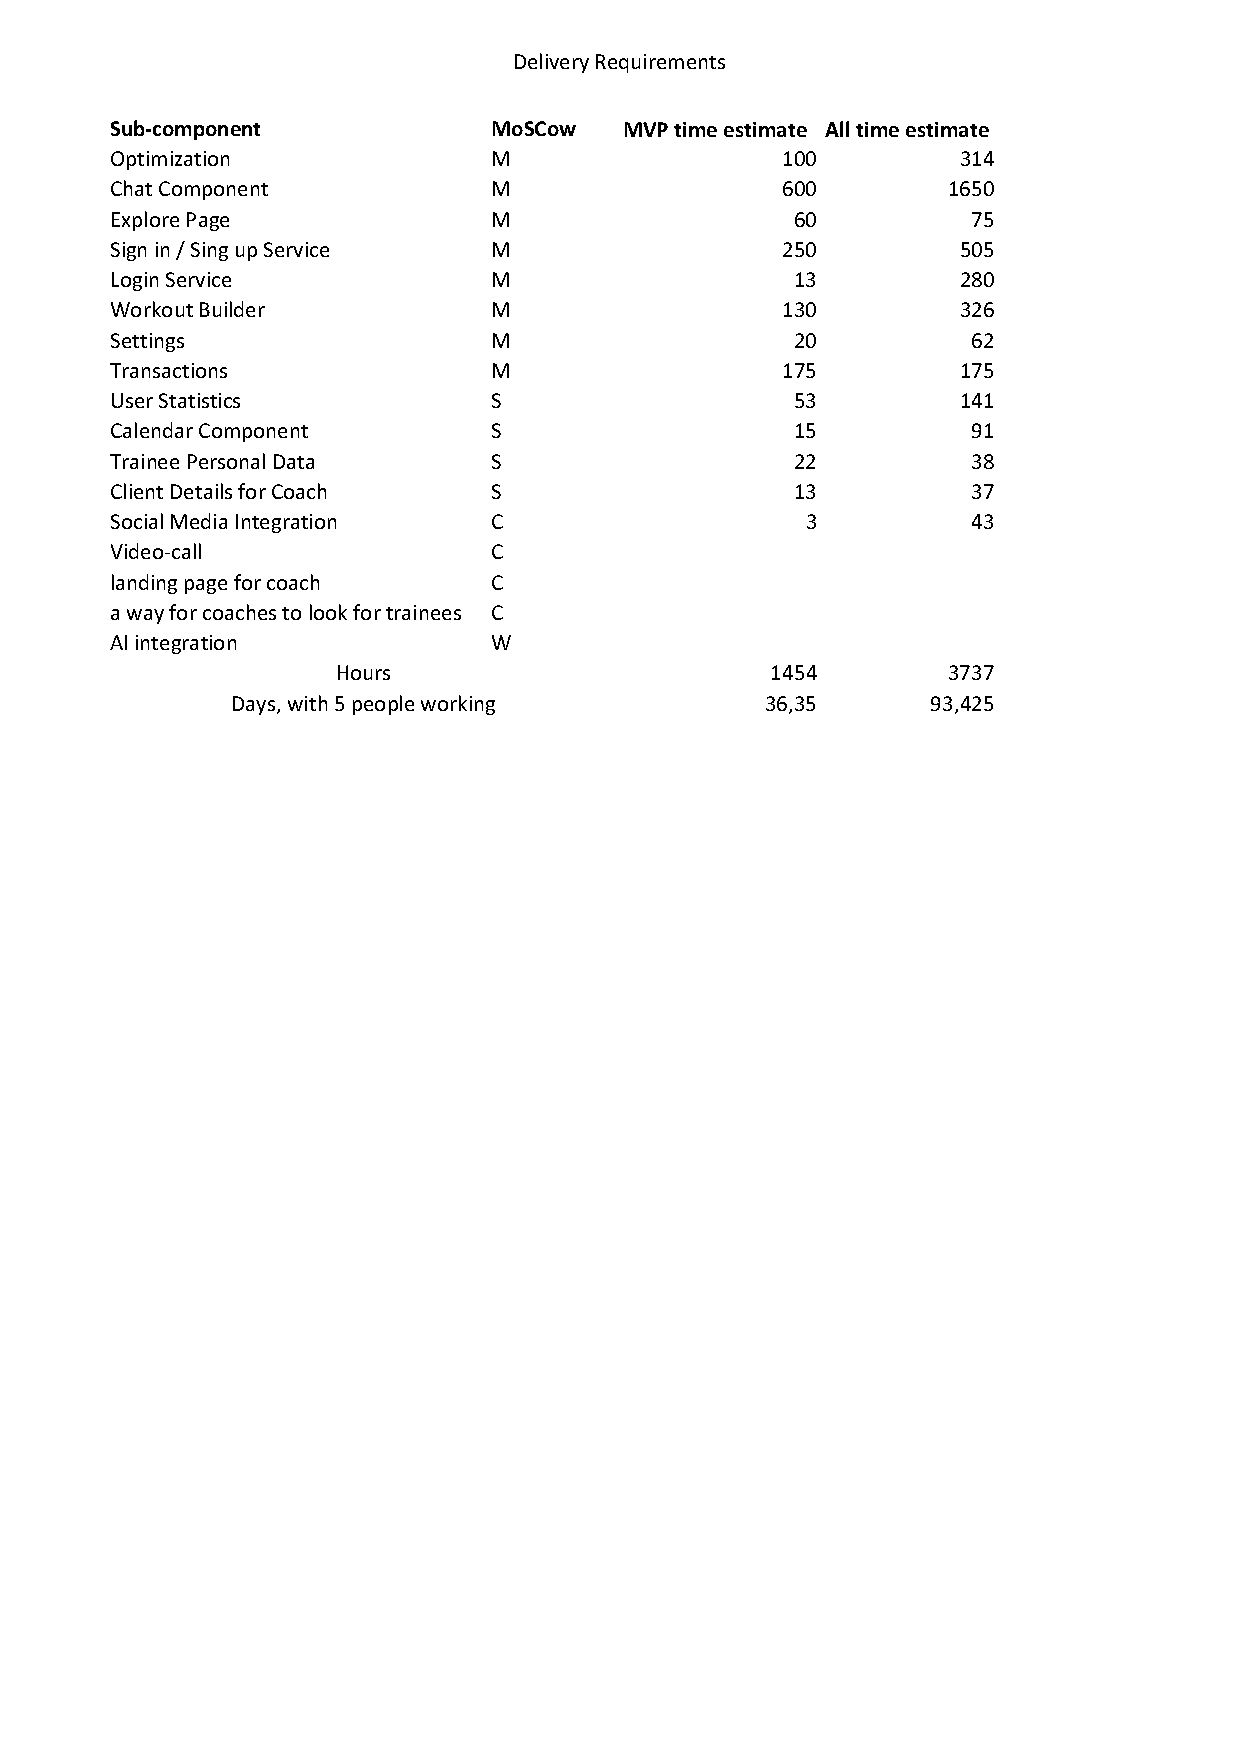
\includepdf[pages=-]{Resources/LinkedGym_requirements_estimates_prio.pdf}